\documentclass[border=12pt]{standalone}
\usepackage[dvipsnames]{xcolor}
\usepackage{amsmath}
\usepackage{tikz}
\usetikzlibrary{arrows.meta,positioning,fit,backgrounds,calc}

% ---------------- colours (matching protograph_construction.tex) ----------------
\definecolor{schemagreen}{RGB}{198,239,206}  % instance / output (green)
\definecolor{ransub}{RGB}{197,233,243}        % relation (cyan)
\definecolor{agentfill}{RGB}{231,222,242}     % class (lavender)
\definecolor{midfill}{RGB}{218,232,247}       % bound / term (blue)
\definecolor{leaffill}{RGB}{244,248,253}      % neighbour / processing (pale blue)
\definecolor{hdr}{RGB}{225,225,225}           % sum node (gray)
\definecolor{darknavy}{RGB}{18,32,86}         % class edges / labels (dark navy)

\newcommand{\ttag}[1]{{\scriptsize\bfseries\textcolor{darknavy}{#1}}}

\begin{document}
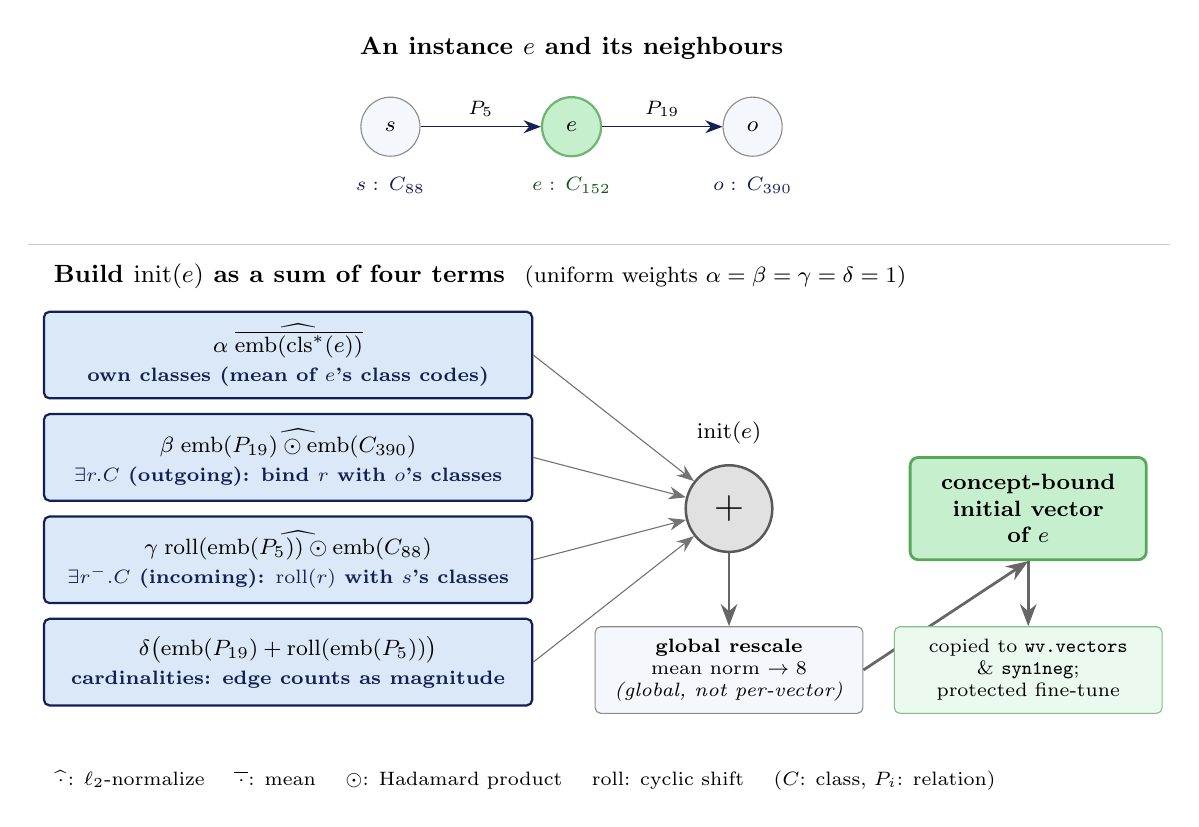
\begin{tikzpicture}[
  font=\footnotesize,
  inst/.style={circle, draw=ForestGreen!65, line width=0.8pt, fill=schemagreen,
               minimum size=7.5mm, font=\footnotesize\bfseries},
  nbr/.style={circle, draw=black!45, fill=leaffill, minimum size=7.5mm, font=\footnotesize},
  edge/.style={-{Stealth[length=2.2mm]}, draw=darknavy},
  term/.style={rounded corners=2pt, draw=darknavy, line width=0.8pt, fill=midfill,
               minimum height=11mm, minimum width=62mm, inner sep=3pt, align=center, font=\footnotesize},
  proc/.style={rounded corners=2pt, draw=black!45, fill=leaffill,
               minimum height=11mm, minimum width=34mm, inner sep=3pt, align=center, font=\scriptsize},
  final/.style={rounded corners=3pt, draw=ForestGreen!75, line width=1pt, fill=schemagreen,
                minimum height=13mm, minimum width=30mm, inner sep=3pt, align=center, font=\footnotesize\bfseries},
  sumn/.style={circle, draw=black!65, line width=0.9pt, fill=hdr, minimum size=11mm, font=\Large},
  arr/.style={-{Stealth[length=2.2mm]}, draw=black!55},
  flow/.style={-{Stealth[length=2.8mm]}, draw=black!60, line width=1pt},
  hdrf/.style={font=\small\bfseries},
]

% ============================================================
% TOP (centred): example neighbourhood of instance e
% ============================================================
\node[hdrf] at (6.6,7.9) {An instance $e$ and its neighbours};
\node[nbr]  (s) at (4.3,6.9) {$s$};
\node[inst] (e) at (6.6,6.9) {$e$};
\node[nbr]  (o) at (8.9,6.9) {$o$};
\draw[edge] (s) -- (e) node[midway, above, font=\scriptsize] {$P_{5}$};
\draw[edge] (e) -- (o) node[midway, above, font=\scriptsize] {$P_{19}$};
\node[font=\scriptsize, text=darknavy]      at (4.3,6.15) {$s:\,C_{88}$};
\node[font=\scriptsize, text=ForestGreen!60!black]  at (6.6,6.15) {$e:\,C_{152}$};
\node[font=\scriptsize, text=darknavy]      at (8.9,6.15) {$o:\,C_{390}$};

% separating rule
\draw[black!20] (-0.3,5.4) -- (14.2,5.4);
\node[hdrf, anchor=west] at (-0.1,5.0)
  {Build $\mathrm{init}(e)$ as a sum of four terms \ \footnotesize\mdseries (uniform weights $\alpha=\beta=\gamma=\delta=1$)};

% ============================================================
% FOUR TERMS (stacked) -> sum
% ============================================================
\def\xt{3.0}
\def\ya{4.0}\def\yb{2.7}\def\yc{1.4}\def\yd{0.1}

\node[term] (pa) at (\xt,\ya)
  {$\alpha\;\widehat{\overline{\mathrm{emb}(\mathrm{cls}^*(e))}}$\\[1pt] \ttag{own classes (mean of $e$'s class codes)}};
\node[term] (pb) at (\xt,\yb)
  {$\beta\;\widehat{\mathrm{emb}(P_{19})\odot \mathrm{emb}(C_{390})}$\\[1pt] \ttag{$\exists r.C$ (outgoing): bind $r$ with $o$'s classes}};
\node[term] (pc) at (\xt,\yc)
  {$\gamma\;\widehat{\mathrm{roll}(\mathrm{emb}(P_{5}))\odot \mathrm{emb}(C_{88})}$\\[1pt] \ttag{$\exists r^{-}.C$ (incoming): $\mathrm{roll}(r)$ with $s$'s classes}};
\node[term] (pd) at (\xt,\yd)
  {$\delta\big(\mathrm{emb}(P_{19})+\mathrm{roll}(\mathrm{emb}(P_{5}))\big)$\\[1pt] \ttag{cardinalities: edge counts as magnitude}};

% sum node
\node[sumn] (sum) at (8.6,2.05) {$+$};
\node[font=\footnotesize, anchor=south] at (8.6,2.75) {$\mathrm{init}(e)$};
\draw[arr] (pa.east) -- (sum);
\draw[arr] (pb.east) -- (sum);
\draw[arr] (pc.east) -- (sum);
\draw[arr] (pd.east) -- (sum);

% rescale -> final -> matrices
\node[proc] (resc) at (8.6,0.0)
  {\textbf{global rescale}\\ mean norm $\to 8$\\ \emph{(global, not per-vector)}};
\draw[flow] (sum) -- (resc);

\node[final] (fin) at (12.4,2.05) {concept-bound\\ initial vector\\ of $e$};
\draw[flow] (resc.east) -- (fin.south);

\node[proc, draw=ForestGreen!55, fill=schemagreen!35] (write) at (12.4,0.0)
  {copied to \texttt{wv.vectors}\\ \& \texttt{syn1neg};\\ protected fine-tune};
\draw[flow] (fin) -- (write);

% ============================================================
% LEGEND
% ============================================================
\node[anchor=west, font=\scriptsize] at (-0.1,-1.4)
  {$\widehat{\,\cdot\,}$: $\ell_2$-normalize \quad $\overline{\,\cdot\,}$: mean \quad $\odot$: Hadamard product \quad $\mathrm{roll}$: cyclic shift \quad ($C$: class, $P_i$: relation)};

\end{tikzpicture}
\end{document}
